\documentclass[tikz,border=3mm]{standalone}
\begin{document}
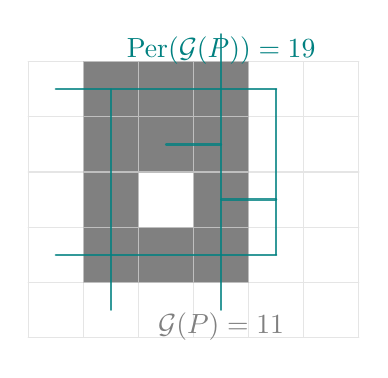
\begin{tikzpicture}[scale=0.7, line cap=round, line join=round]
    % Grid background (optional for visualization)
    \draw[gray!20, thin] (0,0) grid (6,5);
    
    % Cluster definition (11 squares)
    \foreach \coord in {
        (1,1), (1,2), (1,3), (1,4),
        (2,1), (2,3), (2,4),
        (3,1), (3,2), (3,3), (3,4)
    }{
        \draw[fill=gray, draw=gray!50] \coord rectangle +(1,1);
    }
    
    % Perimeter highlighting (19 edges)
    \draw[teal, thick, opacity=0.8] (0.5,1.5) -- (4.5,1.5); % Bottom horizontal
    \draw[teal, thick, opacity=0.8] (0.5,4.5) -- (4.5,4.5); % Top horizontal
    \draw[teal, thick, opacity=0.8] (1.5,0.5) -- (1.5,4.5); % Left vertical
    \draw[teal, thick, opacity=0.8] (3.5,0.5) -- (3.5,5.5); % Middle vertical
    \draw[teal, thick, opacity=0.8] (4.5,1.5) -- (4.5,4.5); % Right vertical
    \draw[teal, thick, opacity=0.8] (2.5,3.5) -- (3.5,3.5); % Internal horizontal
    \draw[teal, thick, opacity=0.8] (3.5,2.5) -- (4.5,2.5); % Internal horizontal
    
    % Annotations
    \node[gray] at (3.5,0.2) {$\abs{\mathcal{G}(P)} = 11$};
    \node[teal] at (3.5,5.2) {$\mathrm{Per}(\mathcal{G}(P)) = 19$};
\end{tikzpicture}
\end{document}